\chapter{RNN}
The remainder of the project focused on creating a Recurrent Neural Network(RNN) for providing those initial probabilities into the Markov model.
Originally the goal was to only use information contained within each word with no sentence wide information at all. This however turned out to
be misguided, as in such a situation there is very little syntactic information to be obtained by purely statistical means.
\section{Proposed Architectures}
On the outset a nonlinear architecture had to be assumed, as 2 outputs are needed. Because of this, several experiments with nonlinear network architectures were performed to gauge which gives best results. All these test were performed on the same English language treebank.
\subsection{Topology 1}
\begin{figure}[h!]
        \centering
        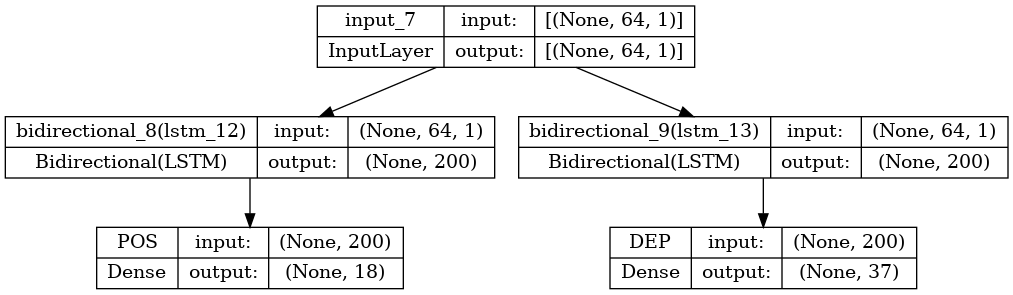
\includegraphics[width=\linewidth]{TOPO/TOPO_3.png}
    \end{figure}
    \clearpage
\subsection{Topology 2}
\begin{figure}[h!]
        \centering
        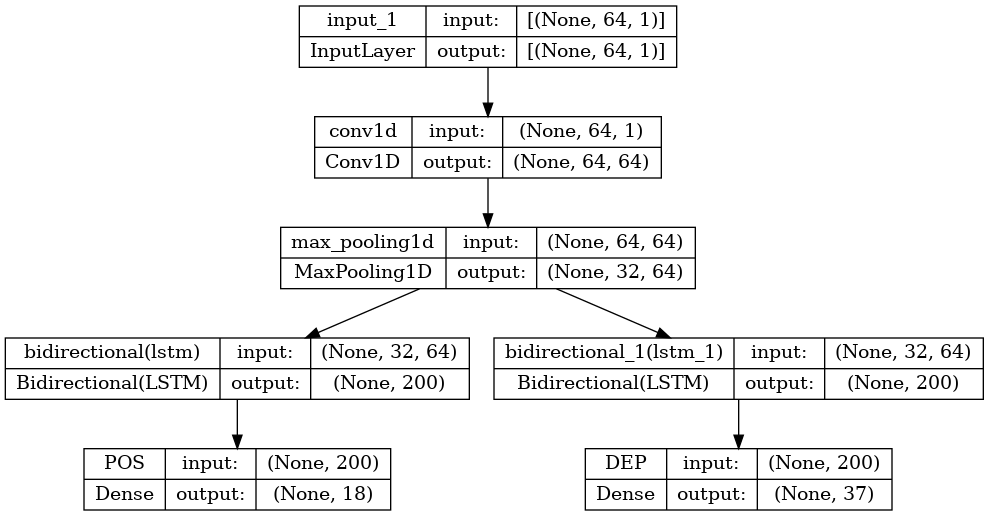
\includegraphics[width=\linewidth]{TOPO/TOPO_2.png}
    \end{figure}
    \clearpage
    \subsection{Topology 3}
    \begin{figure}[h!]
        \centering
        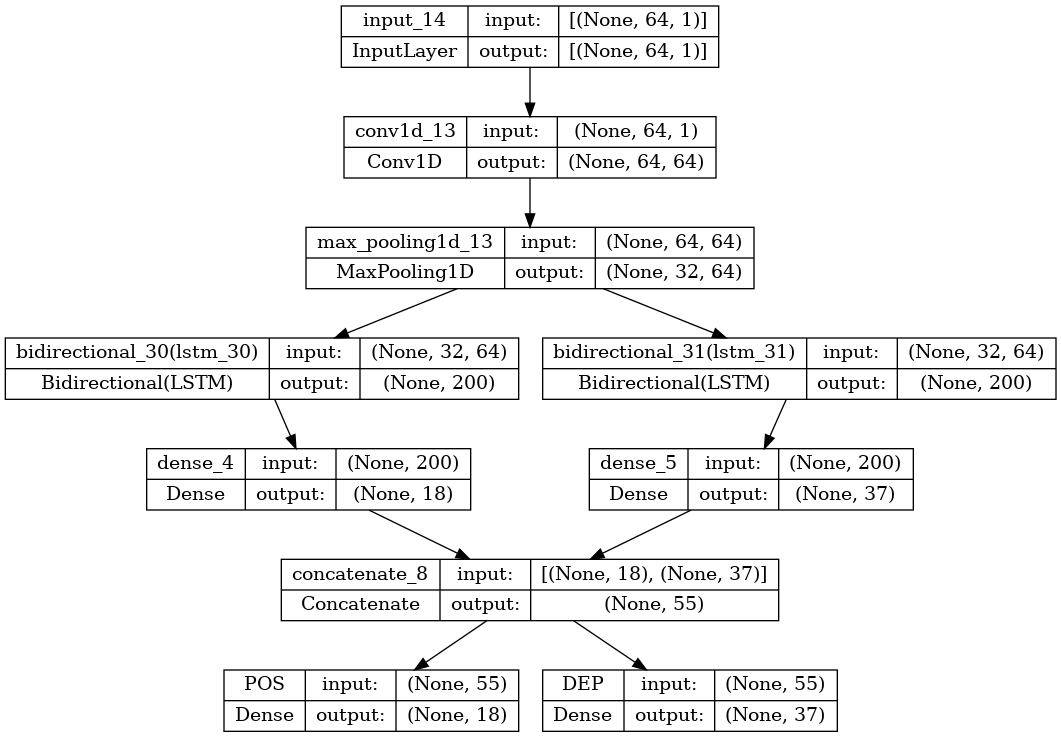
\includegraphics[width=\linewidth]{TOPO/TOPO_1.png}
    \end{figure}
    \section{Overview}
    Of all of the proposed topologies, the first performed the worst, and the 2 others were just a little more than 5\% better at classifying POS and DEP tags.
    The fact that these latter 2 had comparable accuracies was surprising, as that means the network couldn't correlate these different probabilites, or the \\
    correlation was not as strong as one might intuitively suspect. This may however be the result of having split outputs, and hence partially split 
    performance grading.

\section{Convolutional Layer Justification}
The convolutional layer was inserted at the beginning to account for the fact that humans don't perceive language exactly sequentially, as a recurrent neural 
network would. This intuition proved to be correct, as the insertion of this layer gave anywhere from 5\% to 10\% increase in tagging accuracy. Of note is that
while right now only letter combinations are analysed, the same principle holds across word combinations in a sentence. One is very capable of reading even very
jumbled sentences because we perceive words not simply sequentially, but locally.

\clearpage

\section{Results}
The second topology was chosen for further analysis. To test if syntactic information differs across languages, 6 of them were tested.
  \begin{enumerate}
      \item English,
      \item Polish,
      \item French,
      \item Finnish,
      \item German,
      \item Dutch.
  \end{enumerate}\\
The result of this analysis are seen below:
    \begin{table}[h!]
\begin{tabular}{|c|c|c|}
\hline
Language & POS accuracy & DEP accuracy \\ \hline
English  & 0.51         & 0.38         \\ \hline
German   & 0.62         & 0.47         \\ \hline
French   & 0.55         & 0.42         \\ \hline
Finnish  & 0.47         & 0.37         \\ \hline
Polish   & 0.57         & 0.48         \\ \hline
Dutch    & 0.48         & 0.36         \\ \hline
\end{tabular}
\end{table}\\
At first, these results were very surprising. We were expecting for more morphologically complex languages to be easier to classify, but there appeared
to be no trend in that direction. Instead, it appears that the model performed best on languages with many commonly occurring words. German and French both
have gendered articles which appear very commonly and their role in a sentence is very static. This we assume explains the high accuracy observed on these
languages. Confusion matrix for English is provided below(we forgot to take other confusion matrices, but since english also has similar word frequencies, same principle should hold).
\begin{figure}[h!]
        \centering
        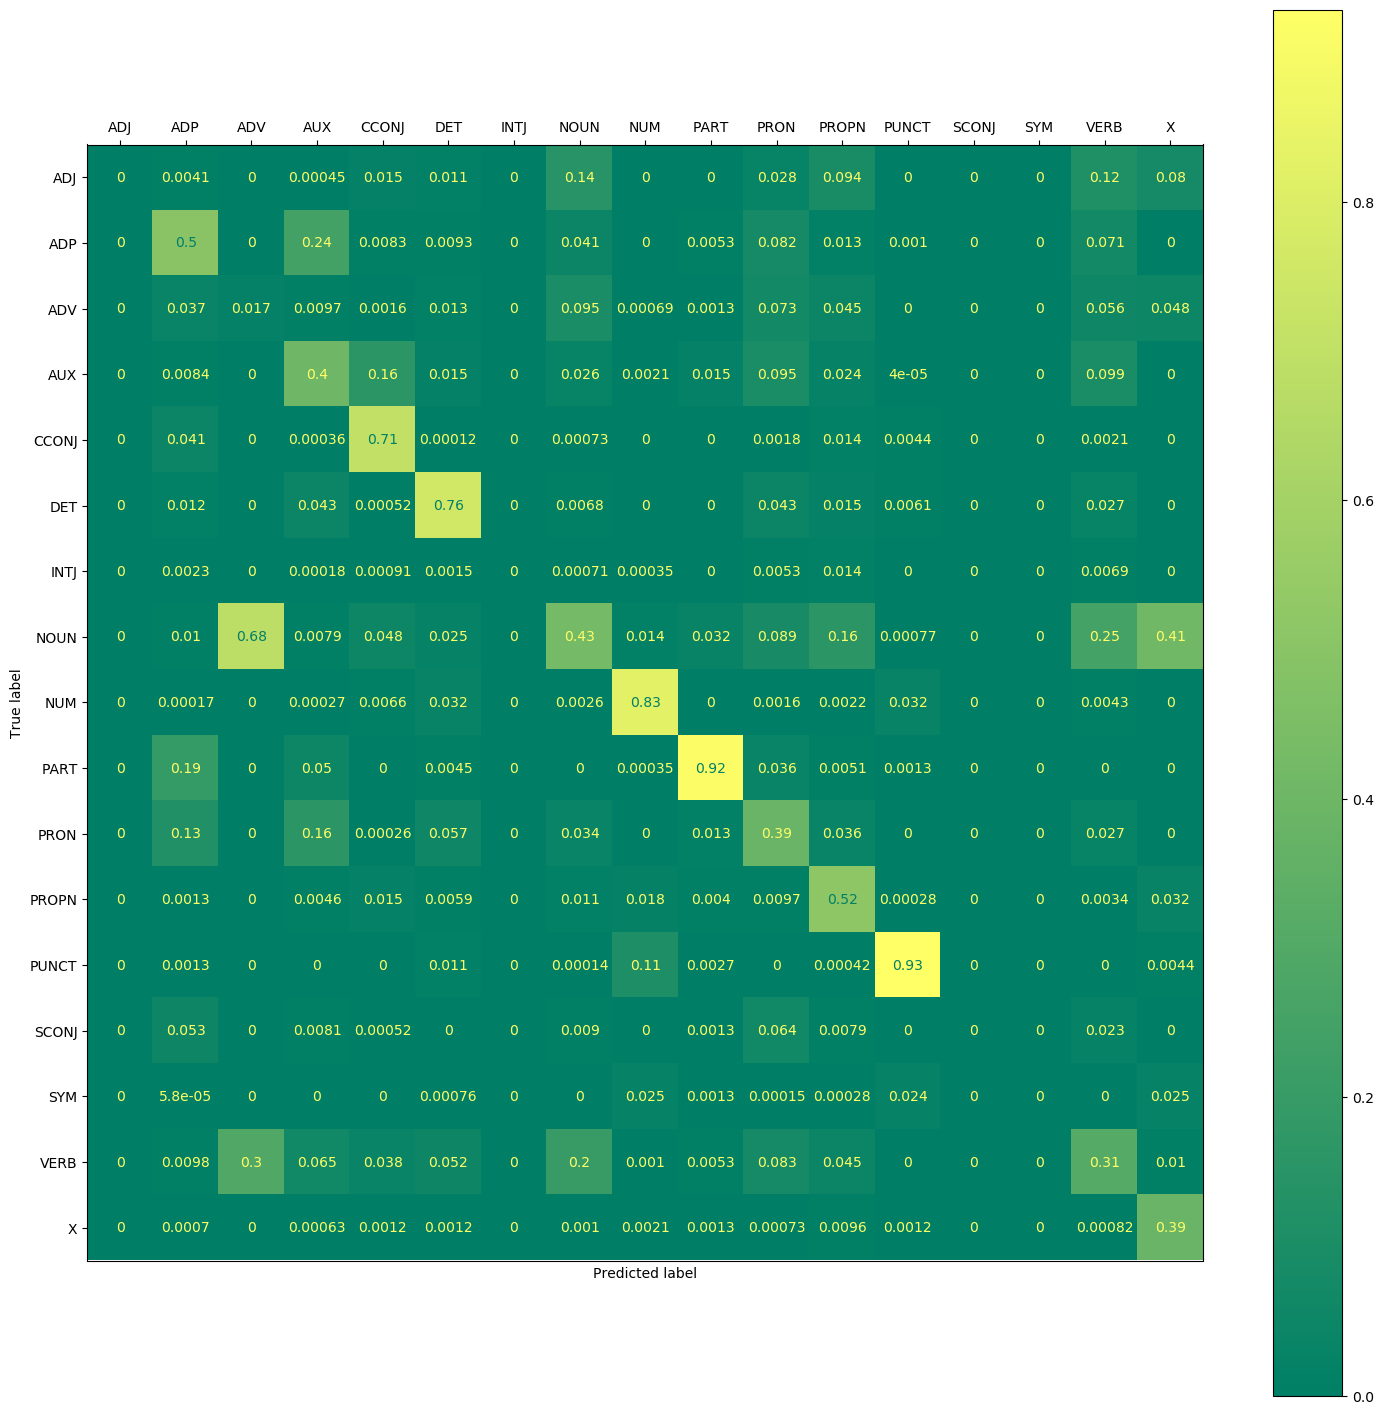
\includegraphics[width=0.5\linewidth]{TOPO/CONF_TOPO_2.png}
\end{figure}\\

We can see, that the POS which were best classified were these that had very few words in them, the DET class for example contains almost only the word "The". Nouns on the other hand were very difficult to classify, as there are very many of them and they can all look very different. 

We can also surmise, that there is a "horizon" of the syntactic knowledge obtainable from a single word. All of the languages tested had their classification probabilities within 15\% of each other, and that around 55\%. This result is not insubstantial, as there are 17 categories to chose from, but the fact that no more can
be extracted just from words hints that syntax is mostly contained in relations between words, and not words themselves.
\subsection{Proposed solution}
As a solution to this problem of classification horizon, we propose a novel architecture which would utilise a double feedback loop between 2 different recurrent layers. The first layer would be responsible for "embedding" words based on their sequence of letters, but it would also receive feedback from the second layer, which
would classify the whole sentence. This way, individual word classifications could use sentence wide information in a sequential manner. The fact that both of these layers are recurrent is very important, as recurrent networks are the only ones which allow for infinite input. Languages can create words and sentences of arbitrary length, so no other type of network can be the basis of a parsing model.

\chapter{Conclusions}
This project turned out to be much more complicated than originally anticipated, and due to this could not be completed in its original form.
The results it provided however could prove very useful in guiding future research, as now there is at least a clear path forward. The proposed
double feedback architecture could be produced in keras, as this library's api allows for creating custom layers from scratch. \\
Most important conclusion to draw from all this, is that stochastic parsing cannot be done just on word based analysis, the whole sentence has
to be taken into account to obtain any useful information.

